\documentclass[12pt]{beamer}
\usepackage{mathtools}
\usepackage{makecell}
\usepackage{caption}
\usepackage{ragged2e}
\usepackage{paralist}
\captionsetup[figure]{labelformat=empty}
\useoutertheme{infolines}
\usetheme{default}
\usefonttheme{serif}
%\usefonttheme{structuresmallcapsserif}
\hypersetup{colorlinks=true,linkcolor=blue}
\setbeamertemplate{navigation symbols}{}
\setbeamertemplate{footline}[frame number]{}
%\setbeamertemplate{footline}{}
\author{Mittereder, \textit{et. al.}}
\definecolor{darkgreen}{rgb}{0,.5,0}
\setlength{\parskip}{.1in}
\newcommand{\freakingtilde}{\raisebox{0.5ex}{\texttildelow}}
\begin{document}

%----------------------------------------------------------------------------
\begin{frame}[c]{}

\begin{center}
\Large

Improving Political Discussion on Social Media
with Automated Bot Intervention

\footnotesize
\textbf{Garrett McKenzie, Bethanie Hackett, Laura Rider}\\
\smallskip
\scriptsize
Faculty advisor: Stephen Davies \\
\medskip
Dept of Computer Science\\
University of Mary Washington\\
Fredericksburg, Virginia, USA\\
\bigskip
\bigskip
\scriptsize
Sixth Annual Network for Undergraduate Research in Virginia (NURVa 2025)\\
\bigskip
\scriptsize
Nov.~1, 2025\\
\texttt{https://github.com/divilian/frozone}
\end{center}

\end{frame}

% counterspeech
% affective polarization
% echo chambers
% political intolerance
% breakdown of trust
%
% * summarize literature on using LLMs as personas (GM)
% * summarize literature on using LLMs to improve political convo (LR)
% * write a concise thesis statement (GM)
% * create architectural images (GM) 
% * make a power point (SD) 
% * make talking points (SD)
% * prepare a demo of ChatGPT with your frobot prompt and hotbot (BH)
% * prepare a "future directions" slide (BH)
% * prepare a "this is what our experiment will do" slide (LR)



%----------------------------------------------------------------------------
\begin{frame}[c]{Politically polarized online conversation}

\small
\begin{center}
Many scholars have observed a degradation in political conversation.
\end{center}

\begin{columns}[c,onlytextwidth]
  \begin{column}{0.2\textwidth}
    \centering
    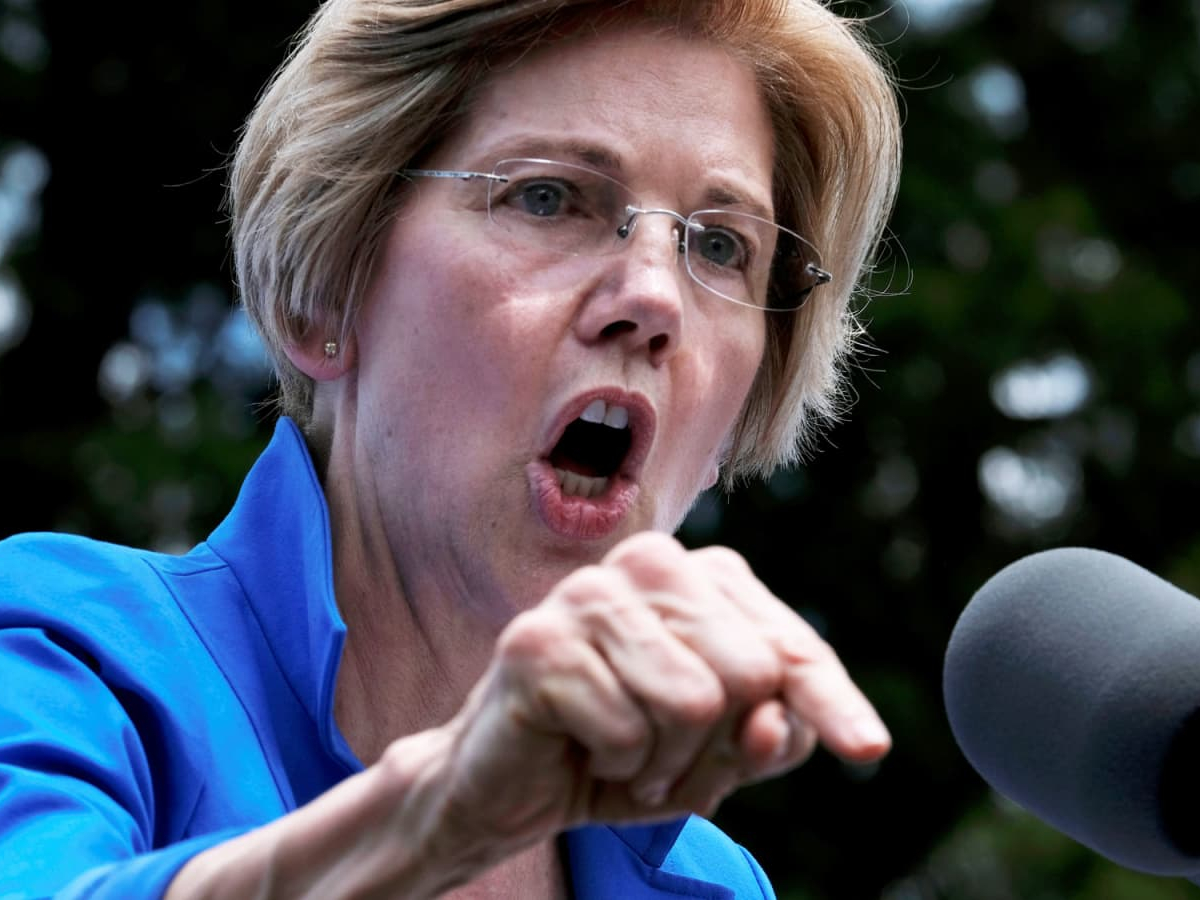
\includegraphics[width=\linewidth]{warren.jpg}\\
    \bigskip
    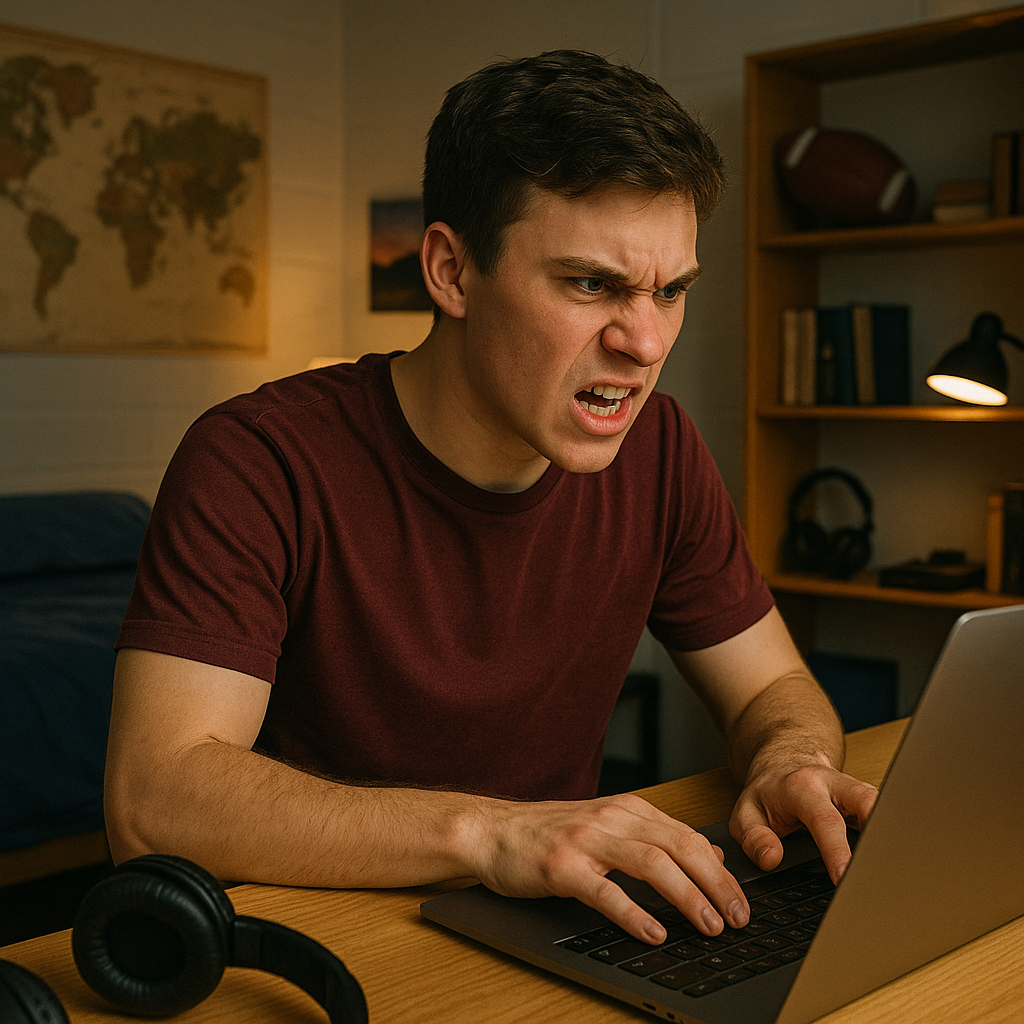
\includegraphics[width=\linewidth]{angryGuy.png}
  \end{column}

  \begin{column}{0.01\textwidth}\hfill\end{column}
  \begin{column}{0.5\textwidth}
  This includes a rise in:\\
    \RaggedRight % optional—keeps bullets from full justification
    \begin{compactitem}
        \item misinformation/disinformation
        \item political intolerance
        \item erroneous reasoning
        \item affective polarization
        \item toxic speech
        \item echo chambers
        \item biased viewpoints
    \end{compactitem}
  \end{column}

  \begin{column}{0.2\textwidth}
    \centering
    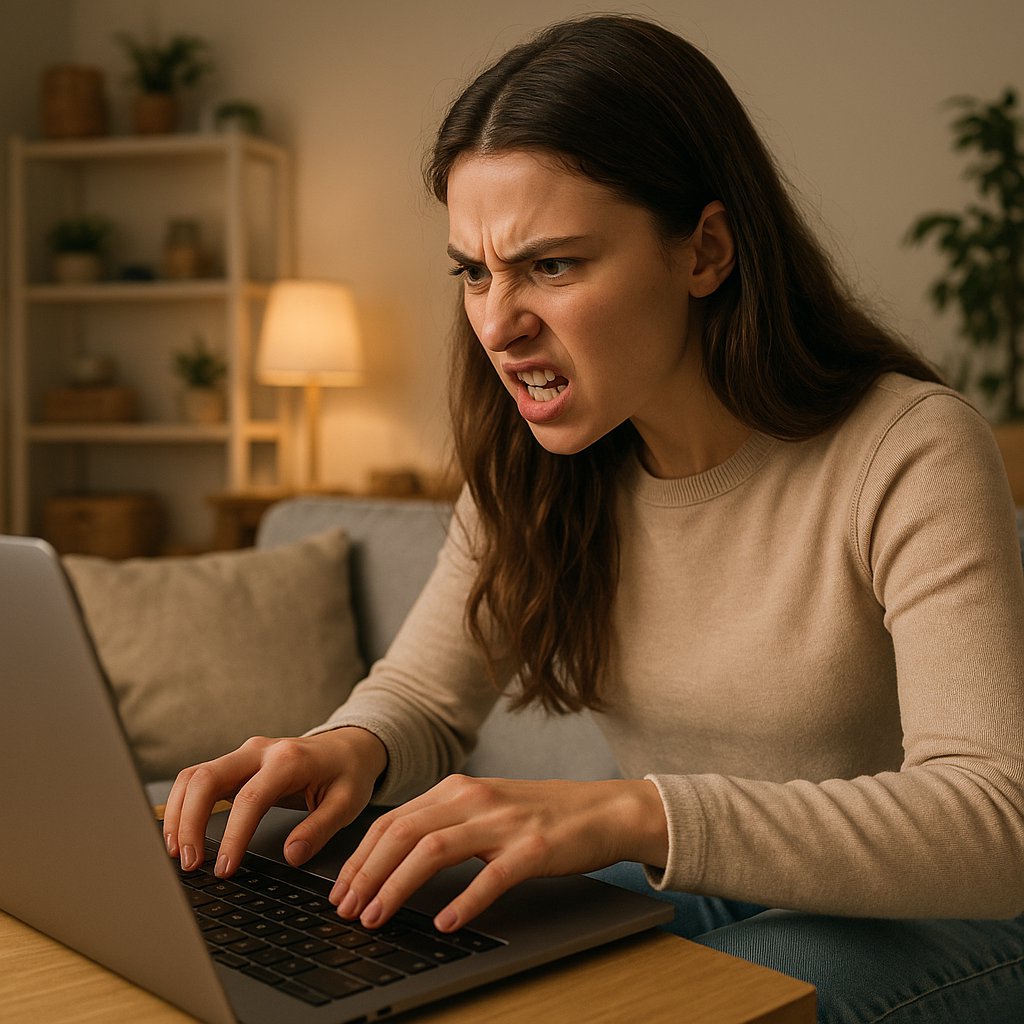
\includegraphics[width=\linewidth]{angryGirl.png} \\
    \bigskip
    
\includegraphics[width=\linewidth]{cruz.jpg}
  \end{column}
\end{columns}

\vspace{-.1in}
\begin{center}
This erosion of trust and communication is alarming for a democracy.\\
\pause
\large Is there a way to improve it?
\end{center}

\end{frame}
%----------------------------------------------------------------------------
\begin{frame}[c]{Main idea}

Train a Large Language Model (LLM) to imitate a human social media participant.

\vspace{-.3in}
\pause

\makebox[\textwidth][c]{%
  \begin{columns}[c,totalwidth=0.7\textwidth]
    \begin{column}{0.3\textwidth}
    \begin{center}
    \LARGE ``FroBot''
    \end{center}
    \end{column}
    \begin{column}{0.7\textwidth}
    
\includegraphics[width=0.4\textwidth]{frozone.png}
    \end{column}
\end{columns}
}

\pause
    
The FroBot will observe and intervene in online conversations:

\small
\begin{compactitem}
\item reduce affective ``temperature''
\item non-threateningly call out misinformation
\item gently identify sources of bias
\item respectfully correct fallacies of reasoning
\end{compactitem}

\end{frame}
%--------------------------------------------
\begin{frame}[c]{Using LLMs as ``personas''}

\footnotesize
\begin{itemize}
\itemsep1em
\item Deshpande, A., Murahari, V., Rajpurohit, T., Kalyan, A., \& Narasimhan, K. (2023). \textbf{Toxicity in chatgpt: Analyzing persona-assigned language models.} In H. Bouamor, J. Pino, \& K. Bali (Eds.), \textit{Findings of the Association for Computational Linguistics: EMNLP 2023} (pp.~1236–1270).

\item Ferraro, A., Galli, A., Gatta, V. L., Postiglione, M., Orlando, G. M., Russo, D., Riccio, G., Romano, A., \& Moscato, V. (2024). \textbf{Agent-Based Modelling Meets Generative AI in Social Network Simulations.} arXiv preprint arXiv:2411.16031.

\item Törnberg, P., Valeeva, D., Uitermark, J., \& Bail, C. (2023). \textbf{Simulating Social Media Using Large Language Models to Evaluate Alternative News Feed Algorithms.} arXiv preprint arXiv:2310.05984.
\end{itemize}


\end{frame}
%----------------------------------------------------------------------------
\begin{frame}[c]{}

\begin{center}
\Large

Improving Political Discussion on Social Media
with Automated Bot Intervention

\footnotesize
\textbf{Garrett McKenzie, Bethanie Hackett, Laura Rider}\\
\smallskip
\scriptsize
Faculty advisor: Stephen Davies \\
\medskip
Dept of Computer Science\\
University of Mary Washington\\
Fredericksburg, Virginia, USA\\
\bigskip
\bigskip
\scriptsize
Sixth Annual Network for Undergraduate Research in Virginia (NURVa 2025)\\
\bigskip
\scriptsize
Nov.~1, 2025\\
\texttt{https://github.com/divilian/frozone}
\end{center}

\end{frame}
%----------------------------------------------------------------------------

\end{document}
